%==============================================================
\newpage

\section{Melodic Similarity}\label{melsimc}

\subsection{Representation}

As presented in section \ref{midiest} there are tools for pitch curve extraction of the main melody line. However in polyphonic music these kind of algorithms struggle to get reasonable results, even in pop music. In musical genres like Metal it gets even worse. In conclusion the main pitch-line extraction and the following conversion of a song with multiple concurrent audio tracks to MIDI using up-to-date open source toolkits doesn't produce very reasonable results as shown in \ref{midiest}.
Another possible representation for melodic features could be to transform the structural information to graphs and use graph comparing algorithms to estimate the similarity between songs. \cite{graph1} 
A better and widely used approach is to use chroma features as described in the next section \ref{chromafeat}.

\subsection{Chroma Features}\label{chromafeat}

Chroma Features as described in section \ref{featsec} are a good and low dimensional way to describe the melodic features of a song. The reduction of dimensionality however comes with a loss of information, especially what octaves the notes are played in. To compute chroma features, most MIR toolkits already offer methods to do so. The plots in this chapter were created using the essentia \cite{essentia1} and librosa \cite{librosa1} toolkits. 
In addition to the pure computation of the chroma features, some pre- and post-processing steps were implemented and tested and will be presented later in this chapter. 
First of all figure \ref{fig:chroma1} shows the chroma feature plots from 2 recordings of the first thirty seconds of the song "Chandelier". Figure a shows the original version sung by the artist Sia and figure b shows the features of a cover version from the band Pvris. 
\begin{figure}[htbp]
	\centering
	\framebox{\parbox{1\textwidth}{ 
			\begin{subfigure}{.495\textwidth}
				\centering 
				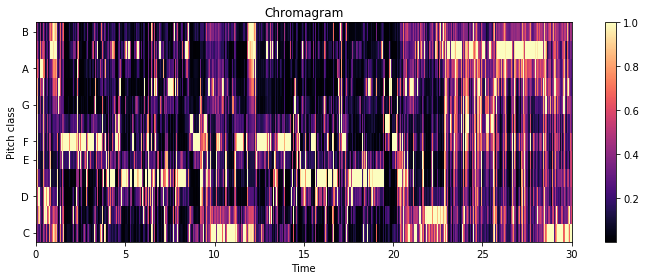
\includegraphics[scale=0.3]{Images/Chroma/sia.png}
				\caption{Chroma Features Sia - Chandelier}
				\label{sia}
			\end{subfigure}%
			\begin{subfigure}{.495\textwidth}
				\centering 
				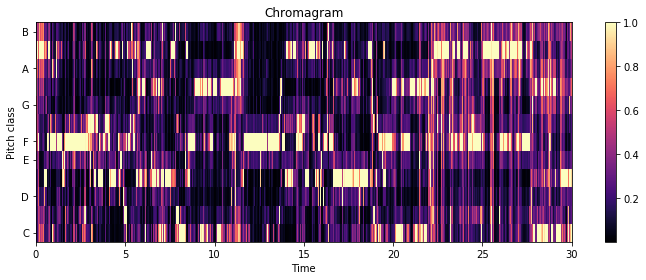
\includegraphics[scale=0.3]{Images/Chroma/pvris.png}
				\caption{Chroma Features Pvris - Chandelier}
				\label{pv}
			\end{subfigure}%	
	}}
	\caption{Chroma Features}
	\label{fig:chroma1}
\end{figure}
In the last third of each sample, the chroma features seemingly get noisier. At these timings in both songs the bass and drum set in. To reduce the effect of rhythm elements over the melodic voice and instrument lines, the audio signal was filtered firstly by a high-pass filter with a cut-off frequency of 128Hz (nearly equal to C3 Key) and secondly by a low-pass filter with a cut-off frequency of 4096Hz (C8 Key). This limits the frequency range to about 5 octaves. 
In figure \ref{fig:sia2} the filter frequency and the original audio signals are visualized in blue color and the filtered audio signal is green. The FFT plot before and after filtering the audio signal is also shown. 
\begin{figure}[htbp]
	\centering
	\framebox{\parbox{1\textwidth}{
			\begin{subfigure}{.495\textwidth}
				\centering
				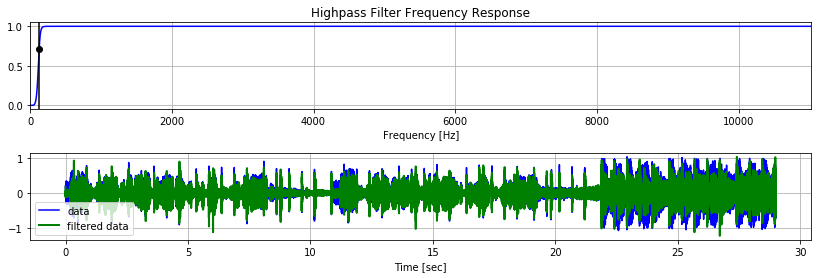
\includegraphics[scale=0.25]{Images/Chroma/siahp.png}
				\caption{Highpassfilter}
				\label{siahp}
			\end{subfigure}%
			\begin{subfigure}{.495\textwidth}
				\centering
				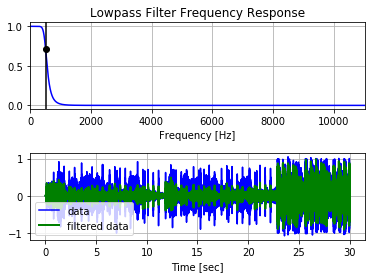
\includegraphics[scale=0.25]{Images/Chroma/sialp.png}
				\caption{Lowpassfilter}
				\label{pvhp}
			\end{subfigure}% 
			
			\begin{subfigure}{.495\textwidth}
				\centering
				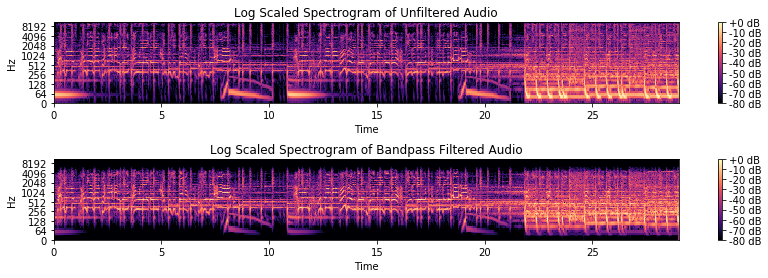
\includegraphics[scale=0.3]{Images/Chroma/siafft.png}
				\caption{FFT Bandpassfilter Sia}
				\label{siafft}
			\end{subfigure}%
			\begin{subfigure}{.495\textwidth}
				\centering
				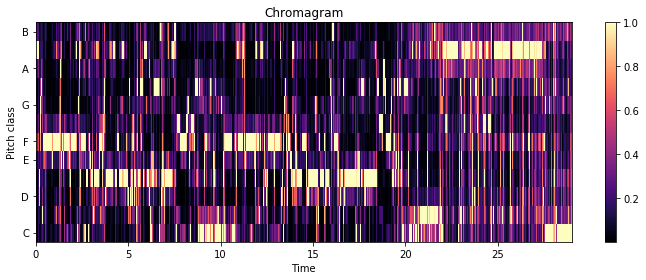
\includegraphics[scale=0.3]{Images/Chroma/chroma_bp.png}
				\caption{Bandpass Filtered Chromagram}
				\label{pvfft}
			\end{subfigure}%			
	}}
	\caption{Bandpass - Sia}
	\label{fig:sia2}
\end{figure}
In the chromagram of the bandpass filtered audio signal the last 10 seconds look cleaner and the melody line is more distinct from the rest in comparison to the chromagram of the unfiltered audio \ref{fig:chroma1}.
The next step is to calculate the most dominant note value for each timeframe. Due to the fact that the chromagram normalizes every timeframe to the maximum note value, the most dominant note always gets the value 1. The closer the rest of the notes are to zero the more likely the timeframe contains silence. If only a few values are close to one, then a chord or harmony is played. To filter out silence the sum over all note values of every timeframe is calculated and if this sum is twice as high as the average sum of notes of the whole song, then the frame is considered as silence. Otherwise the most dominant pitch is set to a fixed value while the rest of the notes are set to zero.\\
To extract the main melody in most cases only the most dominant pitch is needed, but sometimes the main melody is superimposed by other accompanying instruments. To prevent this the second most dominant pitch is also taken into consideration if its value is greater then a specific threshold. 
The result is shown in figure \ref{fig:chromavg} with the threshold 0.8. 
\begin{figure}[htbp]
	\centering
	\framebox{\parbox{1\textwidth}{ 			
			\begin{subfigure}{.495\textwidth}
				\centering    
				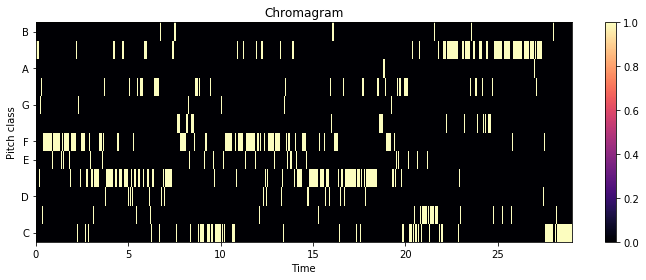
\includegraphics[scale=0.3]{Images/Chroma/sia_1_max.png}
				\caption{Single most dominant note only}
				\label{pvub}
			\end{subfigure}		
			\begin{subfigure}{.495\textwidth}
				\centering     
				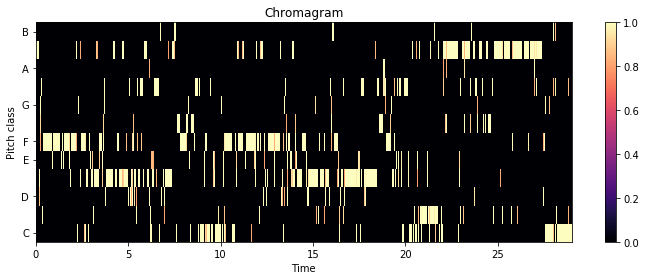
\includegraphics[scale=0.3]{Images/Chroma/sia_2_max.png}
				\caption{First two most dominant notes}
				\label{pvavg}
			\end{subfigure}%			
	}}
	\caption{Thresholded Chroma Features - Sia}
	\label{fig:chromavg}
\end{figure}

After that a beat tracking algorithm is applied to the song and the count of appearances of each note between two beats is calculated. The notes that appear the most are then set 1 while the rest is set to 0 for each section between two beats. This beat-alignment serves to make the similarity measurement invariant to the global tempo of the song. Even if a cover of a song is played with half the tempo of the original song, then the melody of each bar is still the same as in the faster version.
Figure \ref{beataligned} show the different beat aligned features of both songs with bandpass filtered audio and unfiltered audio. The red lines are the detected beat events.
Another option would be to separate the frames between the beats in more smaller sections. This would result in a better resolution of the melodic movement but at the same time increase the length of the data vectors that have to be compared to each other.
\begin{figure}[htbp]
	\centering
	\framebox{\parbox{1\textwidth}{ 			
			\begin{subfigure}{.495\textwidth}
				\centering    
				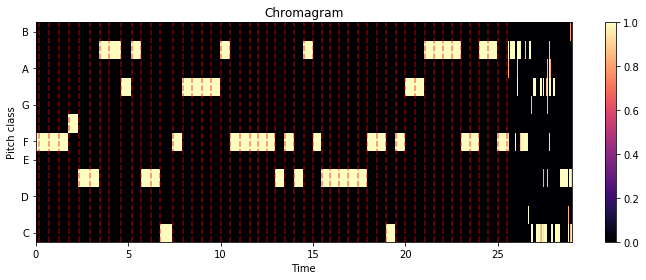
\includegraphics[scale=0.3]{Images/Chroma/pvrisunfiltered.png}
				\caption{Beat aligned of unfiltered audio - Pvris}
				\label{pvubf}
			\end{subfigure}		
			\begin{subfigure}{.495\textwidth}
				\centering     
				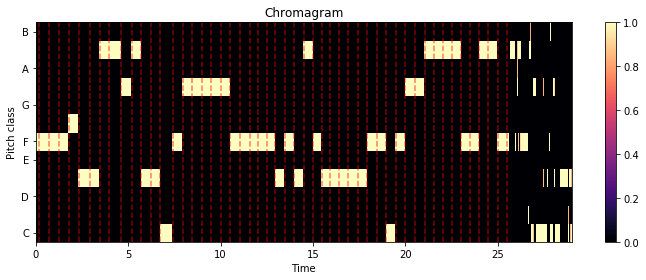
\includegraphics[scale=0.3]{Images/Chroma/pvrisfiltered.png}
				\caption{Beat aligned of filtered audio - Pvris}
				\label{pvfb}
			\end{subfigure}%	
			
			\begin{subfigure}{.495\textwidth}
				\centering    
				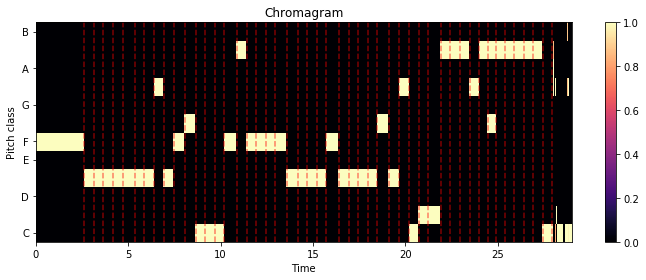
\includegraphics[scale=0.3]{Images/Chroma/siaunfiltered.png}
				\caption{Beat aligned of unfiltered audio - Sia}
				\label{siaub}
			\end{subfigure}
			\begin{subfigure}{.495\textwidth}
				\centering     
				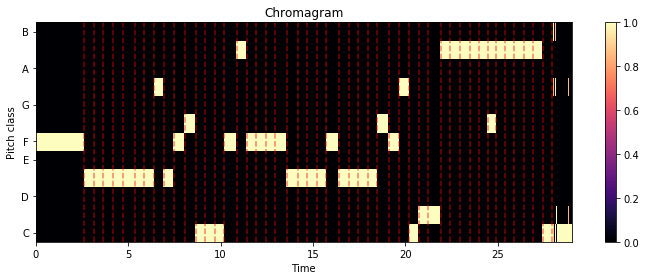
\includegraphics[scale=0.3]{Images/Chroma/siafiltered.png}
				\caption{Beat aligned of filtered audio - Sia}
				\label{siafb}
			\end{subfigure}%		
	}}
	\caption{Processed Chroma Features - Sia}
	\label{beataligned}
\end{figure}
The last processing step is to key shift the chroma features to make the similarity analysis key invariant. One way to do so would be to estimate the key in which the song is played in and then shift all chroma features to the same base key, e.g. C Major or A Minor. Due to the structure of the chroma features this can easily be done by assigning all estimated notes a new value a few keys higher or lower and thus shifting the whole song by a few semitones.\\
The whole workflow to extract the chroma features for this thesis is shown in figure \ref{workflowchrom}.
\begin{figure}[htbp]
	\centering
	\framebox{\parbox{1\textwidth}{ 	
		\centering
		\ \\
		%\smartdiagramset{set color list={blue!40!white, blue!40!white,blue!40!white, blue!40!white, blue!40!white, blue!40!white}}
		\tikzset{priority arrow/.append style={rotate=180,anchor=0,xshift=30,}}			
		\smartdiagram[priority descriptive diagram]{6) key shifting, 5) beat alignment, 4) extract most dominant pitches, 3) filter silence, 2) calculate chromagram, 1) filter audio (bandpass)} \\
		\caption{Workflow chroma feature extraction}
		\label{workflowchrom}
	}}
\end{figure}
%\FloatBarrier
Another consideration is to use the original chromagram without filtering out the least dominant keys and thus leaving the processing step 3 out. This means a possible tradeoff between accuracy and computation time. The result in the example song by Sia doesn't show a major impact, as can be seen in figure \ref{fig:nomax}. In this thesis step 3 will be used in an attempt to get rid of the pitches of the accompaniment from the main melody line.
\begin{figure}[htbp]
	\centering
	\framebox{\parbox{1\textwidth}{ 			
			\begin{subfigure}{.495\textwidth}
				\centering    
				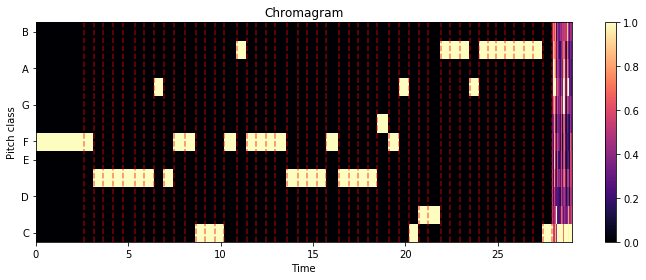
\includegraphics[scale=0.3]{Images/Chroma/nomax.png}
				\caption{Using full chromagram}
				\label{pvubfull}
			\end{subfigure}		
			\begin{subfigure}{.495\textwidth}
				\centering     
				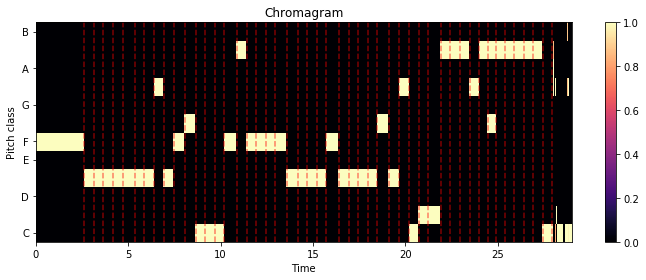
\includegraphics[scale=0.3]{Images/Chroma/siaunfiltered.png}
				\caption{Using most dominant pitches}
				\label{pvdom}
			\end{subfigure}%			
	}}
	\caption{Processing Step 3 Chroma Features}
	\label{fig:nomax}
\end{figure}

\subsection{Similarity of chroma features}

In this section, two completely different approaches to measure the melodic similarity of two songs will be presented. The first one as proposed by \cite{chroma1} or \cite{chroma4} uses text retrieval methods to compare the chroma features of two songs and the second evaluates the usage of cross-correlation as a signal processing approach \cite{chroma2} and \cite{chroma3}

\subsubsection{Text retrieval}

One possibility to process the chromagrams and to estimate similarity between the features of different songs is by handling the features like texts. Due to the extraction of only the main melody line in our feature vector there is only one note for every detected beat. The beat- and pitch-alignment done in the previous steps makes the features relatively time- and key invariant. One problem that remains is the different length of the various feature vectors. \cite{chroma4} mentions that this is indeed a problem when using the levenshtein distance to compute similarity. In their paper they use MIDI files instead of chroma features, but both contain information about the melody of songs so an adaption to chroma features is not an issue, because they can also easily be interpreted as simple strings. The levenshtein distance between the first $i$ characters of a string $S$ and the first $j$ characters of $T$ can be calculated as follows \cite[p. 7]{chroma4}

\begin{equation} \label{eq:tr1}
lev_{S,T}(i, j) = \begin{cases}
max(i, j), &\text{if } min(i, j) = 0\\
min \begin{cases}
lev_{S,T}(i-1, j) + 1\\
lev_{S,T}(i, j-1) + 1\\
lev_{S,T}(i-1, j-1)\\
+cost[S_i \neq T_j]\\
\end{cases} &\text{else} \\
\end{cases}
\end{equation}
Xia (et al.) made some adjustments to this to be able to handle musical information.\cite[pp. 7ff]{chroma4} For example to get rid of the problem of various lengths between the songs, they only took the first 200 and the last 200 notes of every song because it could be observed that cover songs tend to share more common notes in the beginning and in the end of each song.\\
Due to the fact that this thesis has no actual note information from MIDI files but rather short lists of estimated main pitches from the beat aligned chroma features, most of the feature vectors are already smaller than 200 notes. Therefor the implemented algorithm does not split the vectors. This tends to favor cover songs that share the same length. 
\ \\
Englmeier  (et al.) use more advanced information retrieval techniques called TF-IDF weights and explicit semantic analysis (ESA). "The TF-IDF weight is a measure which expresses the meaning of a term or a document within a collection of documents." \cite[p. 186]{chroma1}
To do so, they have to create "audio words" from the song database by splitting the audio signal into snippets, creating chroma features and clustering them with the k-means algorithm. The centroids are then added to a database. These audio words can then be evaluated using the TF-IDF weights and ESA.
Although their approach looks promising, a re-implementation of their algorithms would exceed the frame of this thesis.

\subsubsection{Cross-correlation}

Another possibility to handle the extracted chroma features is by viewing them as ordinary signals and creating opportunities to apply classical signal processing algorithms. Ellis and Poliner use cross-correlation in their 2007 published paper \cite{chroma3}. Serra (et al.) also reference the work of Ellis and Poliner and discuss different weak points and influences of processing steps like beat tracking and key transposition to the overall performance of this similarity measurement. 
They also discuss and improve an other approach called dynamic time warping (DTW) further in their paper \cite{chroma2}. The focus in this thesis is set on the cross-correlation method. 
Given two discrete time signals $x[n]$ and $y[n]$ the cross-correlation between the both signals $k[n] = (x \star y)[n]$ can be denoted as follows:
\begin{equation} \label{eq:conv1}
k[n] = (x \star y)[n] = \sum_{m = -\infty}^{\infty}{x[m] y[m - n]} 
\end{equation}
For two 2-dimensional input matrices $X$ with the dimensions $M$ by $N$ and $Y$ as an $P$ by $Q$ matrix the cross-correlation result is a matrix $C$ of size $M + P - 1$ rows and $N + Q - 1$ columns. Its elements are given by equation \ref{eq:conv2} \cite{mathcorr}, the bar over H denotes complex conjugation (in this case H is a matrix with real values only).
\begin{equation} \label{eq:conv2}
C(k, l) = \sum_{m = 0}^{M - 1}{\sum_{n = 0}^{N - 1}{X(m, n)\overline{H}(m - k, n - l)}}
\end{equation}
with 
\begin{equation} \label{eq:conv3}
-(P - 1) \leq k \leq M - 1
\end{equation}
\begin{equation} \label{eq:conv4}
-(Q - 1) \leq l \leq N - 1
\end{equation}
An example for the one dimensional cross-correlation is shown in figure \ref{fig:corr1} and the full two dimensional cross-correlation of two songs is figured in figure \ref{fig:beatalign} and \ref{fig:crosscorr}.
\begin{figure}[htbp]
	\centering
	\framebox{\parbox{1\textwidth}{ \centering			
	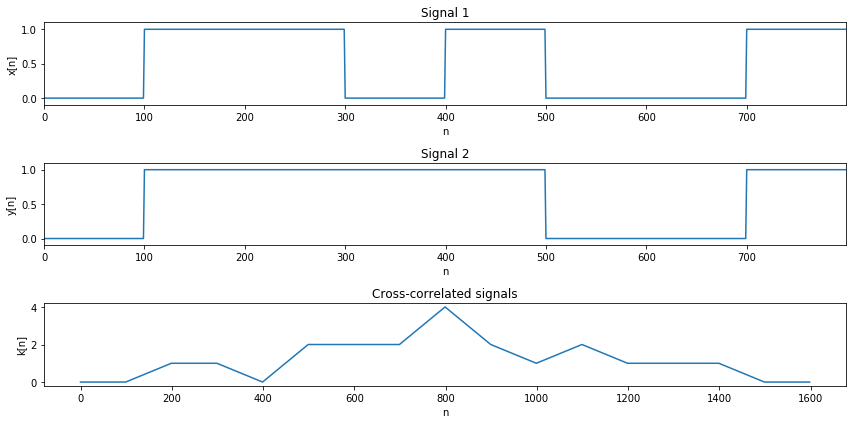
\includegraphics[scale=0.45]{Images/Chroma/correlation.png}
	}}
	\caption{cross-correlation}
	\label{fig:corr1}
\end{figure}
Ellis and Poliner did not transpose the songs in the pre-processing step to match the keys of both audio files. Instead they calculated the full cross-correlation for all 12 possible transpositions and chose the best one. 
As input matrices they averaged all notes of the chroma features per beat and scaled them to have unit norm at each time slice/ beat frame.
In the original paper the cross-correlation is normalized by the length of the shorter song segment to bind the correlation result to an interval between 0 and 1. But in a later published work from Ellis and Cotton this step was left out, as it seemingly resulted in slightly worse detection ratios of cover songs \cite{cover802}. 
Additionally they filtered the result of the correlation with a high-pass filter. "We found that genuine matches were indicated not only by cross-correlations of large magnitudes, but that these large values occurred in narrow local maxima in the cross-correlations that fell off rapidly as the relative alignment changed from its best value. To emphasize these sharp local maxima, we choose the transposition that gives the largest peak correlation then high-pass filter that cross-correlation function with a 3dB point at 0.1 rad/sample" \cite[p. 1431]{chroma3}. The later published paper \cite{cover802} also states, that changes to the filter parameters improved the cover song recognition rate further, however the exact values e.g. for the cutoff frequency weren't give, so this thesis uses the older parameters for the filter\\
Serra (et al.) discussed various effects of pre-processing steps that improve the algorithm even more. E.g they note that a higher chroma resolution of 3 octaves gives better results. Also a key detection and transposition before cross-correlation gives slightly worse results in comparison to the method Ellis and Poliner used.\\ 
In this thesis a versions where the songs are all key aligned before the cross-correlation was tested, but due to the fact, that the key detection algorithm in the labrosa and essentia frameworks weren't always correct a second version where addionally the cross-correlation for all key transpositions is calculated, was also implemented. 
In summary, the implementation in this thesis is similar to the approach by Ellis and Poliner \cite{chroma3} but some of the steps from the newer paper \cite{cover802} leave some room for further improvements.\\ The chroma features are beat aligned, averaged per beat and normalized to unit length as well. Additionally all chroma features are transposed to a common key (A in this case) in the pre-processing step. The full cross-correlation according to equation including key shifts by letting $k$ run from $-(P - 1) \leq k \leq M - 1$ in equation \ref{eq:conv2} is shown in the figures \ref{fig:beatalign} and \ref{fig:crosscorr} but due to the previous pre-processing key shift and the fact that both input matrices share the same amount of rows (12, one per key) these aren't ultimately necessary and computation time can be safed by altering the equation to equation \ref{eq:conv5} resulting in a vector C with the correlation results without additional key-shifting but this version is reliant on an accurate key detection of the songs.
\begin{equation} \label{eq:conv5}
C(l) = \sum_{m = 0}^{M - 1}{\sum_{n = 0}^{N - 1}{X(m, n)\overline{H}(m, n - l)}}
\end{equation}
\begin{equation} \label{eq:conv6}
-(Q - 1) \leq l \leq N - 1
\end{equation}
or even faster without calculating the edges of the matrix.
\begin{equation} \label{eq:conv7}
0 \leq l \leq N - Q
\end{equation}
The post-processing step from Ellis and Poliner, namely the high-pass filtering of the result was also implemented.\\
Figure \ref{fig:beatalign} shows two beat aligned, key shifted and per beat averaged chroma features of two short guitar snippets and their cross-correlation. The interesting row of the cross-correlation matrix is the middle row marked with the C key. It shows that both already key shifted melodies do not correlate well.  
\begin{figure}[htbp]
	\centering
	\framebox{\parbox{1\textwidth}{ 			
			\begin{subfigure}{.495\textwidth}
				\centering    
				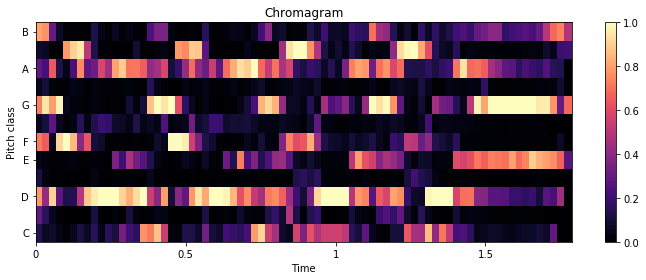
\includegraphics[scale=0.3]{Images/Chroma/beatalignedchroma.png}
				\caption{beat aligned chroma sound1}
				\label{c1}
			\end{subfigure}				
			\begin{subfigure}{.495\textwidth}
				\centering    
				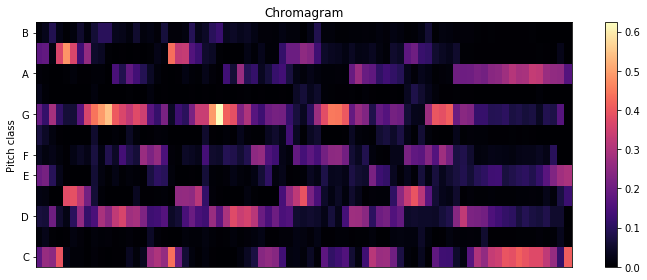
\includegraphics[scale=0.3]{Images/Chroma/beatalignedchroma_ks.png}
				\caption{beat aligned chroma sound1 key shifted}
				\label{cks1}
			\end{subfigure}		
			
			\begin{subfigure}{.495\textwidth}
				\centering     
				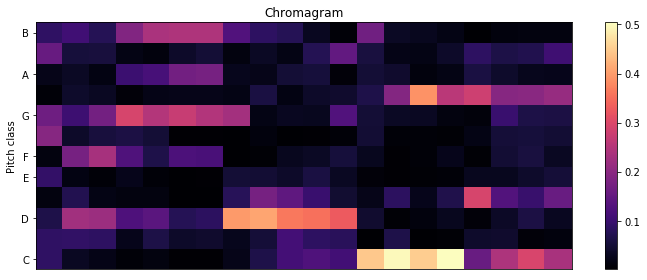
\includegraphics[scale=0.3]{Images/Chroma/beatalignedchroma2_ks.png}
				\caption{beat aligned chroma sound2 key shifted}
				\label{cks2}
			\end{subfigure}%	
			\begin{subfigure}{.495\textwidth}
				\centering     
				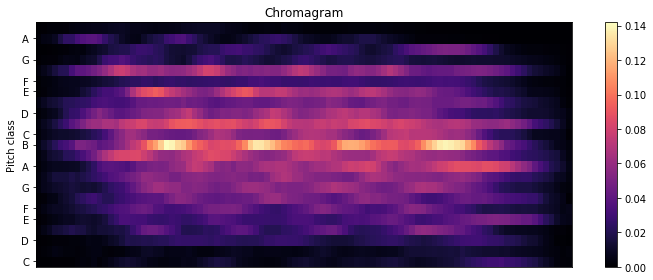
\includegraphics[scale=0.3]{Images/Chroma/beatalignedchroma_corr.png}
				\caption{cross-correlation}
				\label{c2}
			\end{subfigure}%			
	}}
	\caption{beat-aligned chromagram}
	\label{fig:beatalign}
\end{figure}
In figure \ref{fig:crosscorr} the cross-correlation of the song "Chandelier" by the singer Sia and covered by Pvris are shown in \ref{cc1} and in contrast to this the cross-correlation of "Rock you like a Hurricane" with the song "Chandelier" by Sia are shown. Due to the previous key shifting, plot \ref{cch1} shows the maximum peak right in the center row. Originally the version by Sia is detected to be written in C sharp and the cover version in F sharp, but both songs are shifted to the A key in the pre-processing step.\\
The unrelated songs result in much smaller correlation values, especially when looking at the middling row of the matrix (marked as the B-key), but also if the songs are transposed additionally even then they do not correlate well. In contrast to this the cover songs have multiple visible peaks in the center row. 
\begin{figure}[htbp]
	\centering
	\framebox{\parbox{1\textwidth}{ 			
			\begin{subfigure}{.495\textwidth}
				\centering    
				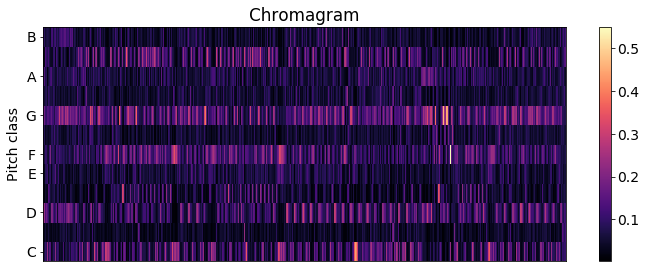
\includegraphics[scale=0.3]{Images/Chroma/hurr1chrom.png}
				\caption{Pvris}
				\label{cch1}
			\end{subfigure}		
			\begin{subfigure}{.495\textwidth}
				\centering     
				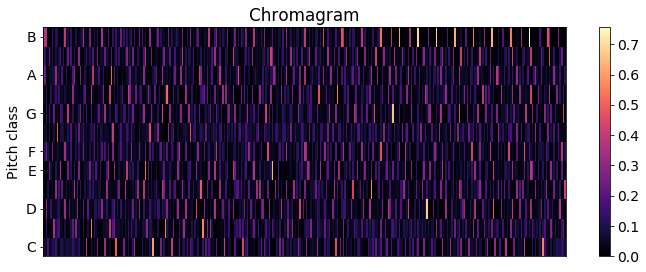
\includegraphics[scale=0.3]{Images/Chroma/hurr2chrom.png}
				\caption{Sia}
				\label{cch2}
			\end{subfigure}%
				
			\begin{subfigure}{.495\textwidth}
				\centering    
				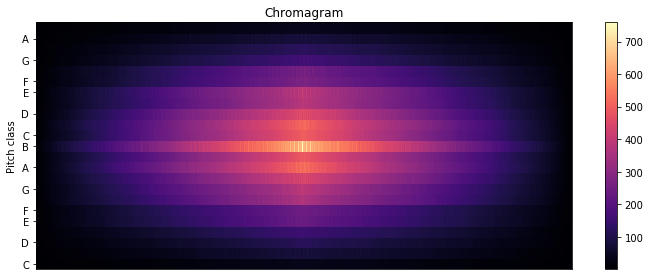
\includegraphics[scale=0.3]{Images/Chroma/cross_hurricane.png}
				\caption{cross-correlation of cover songs}
				\label{cc1}
			\end{subfigure}		
			\begin{subfigure}{.495\textwidth}
				\centering     
				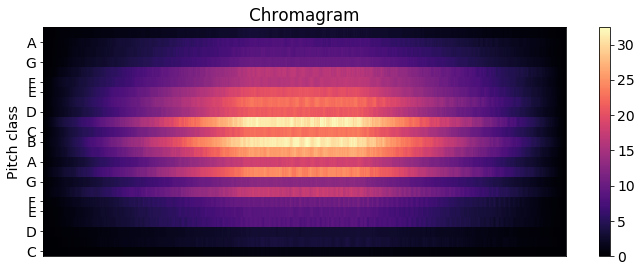
\includegraphics[scale=0.3]{Images/Chroma/cross_hurricane_sia.png}
				\caption{cross-correlation of unrelated songs}
				\label{cc2}
			\end{subfigure}%			
	}}
	\caption{Cross-correlation}
	\label{fig:crosscorr}
\end{figure}
The row with the maximum correlation value is extracted and the resulting plot shows, that the cover songs do correlate much better than the unrelated songs (\ref{cc3} and \ref{cc4}).
The center rows of the cross-correlation matrices from figure \ref{fig:crosscorr} are separately pictured in figure \ref{fig:crosscorr2} and \ref{fig:crosscorr3}. After applying the high-pass filter to the extracted row with the maximum correlation value, the peaks in \ref{cc3} when cross-correlating the cover songs is clearly visible compared to the unrelated songs. An interesting detail that can be pointed out is that the song structure is also visible in plot \ref{ccf3} with clearly visible recurring peaks when the refrain is repeated.
\begin{figure}[htbp]
	\centering
	\framebox{\parbox{1\textwidth}{ 			
			\begin{subfigure}{.495\textwidth}
				\centering    
				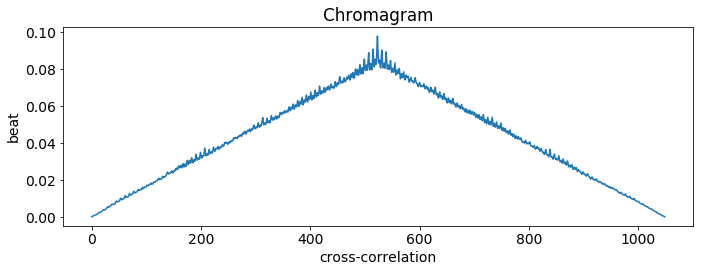
\includegraphics[scale=0.3]{Images/Chroma/beatalignedchroma_corr_mean.png}
				\caption{cross-correlation of cover songs}
				\label{cc3}
			\end{subfigure}		
			\begin{subfigure}{.495\textwidth}
				\centering     
				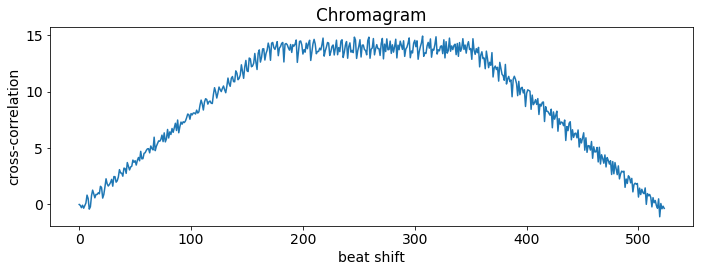
\includegraphics[scale=0.3]{Images/Chroma/beatalignedchroma_corr_mean2.png}
				\caption{cross-correlation of unrelated songs}
				\label{cc4}
			\end{subfigure}%			
	}}
	\caption{Cross-correlation}
	\label{fig:crosscorr2}
\end{figure}
\FloatBarrier

\begin{figure}[htbp]
	\centering
	\framebox{\parbox{1\textwidth}{ 				
			\begin{subfigure}{.495\textwidth}
				\centering    
				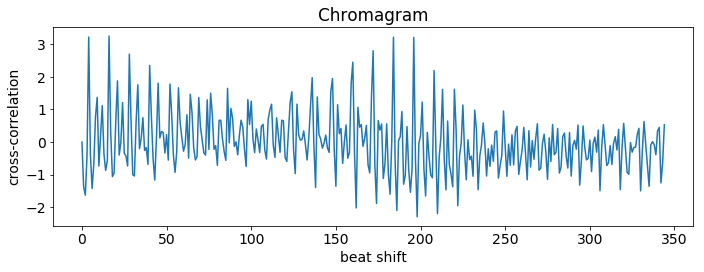
\includegraphics[scale=0.3]{Images/Chroma/beatalignedchroma_corr_mean_filt.png}
				\caption{cover songs filtered}
				\label{ccf3}
			\end{subfigure}		
			\begin{subfigure}{.495\textwidth}
				\centering     
				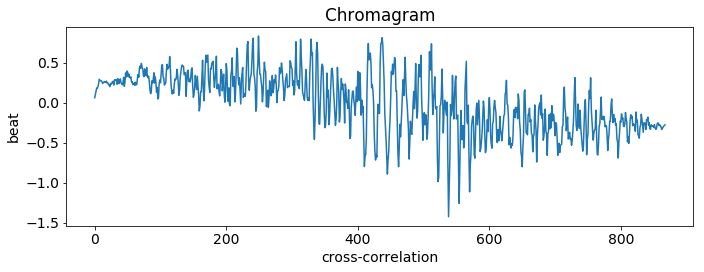
\includegraphics[scale=0.3]{Images/Chroma/beatalignedchroma_corr_mean2_filt.png}
				\caption{unrelated songs filtered}
				\label{ccf4}
			\end{subfigure}%		
	}}
	\caption{Cross-correlation filtered}
	\label{fig:crosscorr3}
\end{figure}
\FloatBarrier



\subsection{Validation}
A good measure for the efficiency of a melodic similarity algorithm is the ability to find cover songs, remixes and recordings of the same song from different artists. 
